\chapter[][State of the Art]{High frequency wedge diffraction models}
\label{chap-biblio}

\section*{Introduction}
\acrfull{ndt} of industrial structures requires the modeling of specimen geometry echoes generated by the surfaces (entry, back-wall...) of inspected blocks. If these surfaces contain wedges, it is then necessary to provide a correct model of the interaction between the ultrasonic beam and these wedges. These interactions may be linked to two different phenomena : reflection from the wedge faces and diffraction of the incident rays by the wedge edge. Both must be correctly taken into account by the model. For that purpose, the study of plane elastic wave diffraction by a wedge is of great interest since surfaces of complex industrial specimen often include dihedral corners.
These inspections often deal with high frequency ($f=2-5$ MHz) ultrasonic waves. A study of the existing models for the problem of wedge diffraction shows that the \acrfull{ge} model (a ray-tracing method based on geometrical optics) developed by CEA/LIST and partners in the \acrshort{ndt} simulation platform CIVA \cite{Darmonspec} is much faster than other numerical models (finite elements or finite differences for example) because such methods require a small mesh step (of the order of a third or a fifth of the wavelength) for a better description of the scattered wave. However, this model computes reflection but not diffraction. To complete this model, the \acrfull{gtd} was developed by Keller \cite{GTD} in optics and extended to elastic waves by Achenbach and Gautesen \cite{AchenbachGautesen, Achenbach}. However, this model is not spatially uniform in the sens that it diverges in certain directions. 

The \acrfull{ka} was first developed in optics \cite{POoptics} before being used for \acrshort{ndt} applications \cite{Schmerr,Dorval}. It is a high-frequency uniform scattering model but can be inaccurate far from directions of geometrical reflection. To overcome this shortcoming, an ultrasonic system model based on the \acrfull{ptd} introduced by Ufmitsev \cite{Ufmi} has been developed for a half-plane by Zernov et al. \cite{Zernov} and extended to mimic ultrasonics with some head waves \cite{systmodel,FradkinDarmon}. Nevertheless, this ultrasonic \acrshort{ptd} model can be time consuming for large specimen surfaces. A third solution to this problem, called the \acrfull{uat} was proposed for elastic waves by Achenbach et aL. \cite{Achenbach}. This method models diffraction well but is difficult to implement for complex geometries. Finally, the \acrfull{utd} was proposed in elastodynamics by Kamta Djakou et al. \cite{Audrey, AKDthese} and developed for a half-plane scatterer and for a wedge. It combines the specular model with a diffraction model. Our future idea is to extend \acrshort{utd} to the wedge case, which needs the development of a robust wedge diffraction model. To apply the aforementioned \acrshort{utd} method, a generic and trustworthy wedge diffraction model is necessary.

Section 1 of this chapter presents the two non-uniform scattering models : the \acrshort{ge} model and the \acrshort{gtd} model. Section 2 describes the proposed uniform corrections of these models. The advantages and inconveniences of each of these models are also discussed. Finally, section 3 details two semi-analytical computation methods for the problem of 2D elastic wave diffraction by a stress-free wedge.

\section{Non-Uniform asymptotic methods}

There are various high-frequency approximations of the field echoed by the surfaces and interfaces of an inspected specimen. Some of these models lead to a discontinuous scattered field (which is not physical) and are therefore called non-uniform methods, as opposed to uniform models, which lead to continuous solutions.
\subsection{\acrfull{ge}}
\label{sectGE}
The first approximation that can be applied to the study of wave propagation in a complex isotropic medium is the \acrfull{ge} model. It is a translation to elastodynamics of the geometrical optics theory. The field's propagation is described by ray tracing, each ray carrying a certain field value. At a given observation point, the field's value is the sum of the values carried by each of the rays passing through this point. In the \acrshort{ge} theory, the incident, reflected and refracted rays are described. These rays are computed following Snell's laws of reflection and refraction :
\begin{equation}
    \frac{1}{c_{\alpha}}\cos\theta_{\alpha} = \frac{1}{c_{\beta}} \cos\theta_{\beta}
    \label{Snellrefl}
\end{equation}
In all this thesis, $\alpha=L,TH$ or $TV$ represents the type of the incident wave (L for Longitudinal, TH for Transverse Horizontal and TV for Transverse Vertical) and $\beta$ is the type of the reflected, transmitted of diffracted wave.

When the incident wave meets a surface containing an edge, the propagation medium can be decomposed into four zones (see Fig.~\ref{illuzones}) :
\begin{itemize}
	\item Zone I : the incident rays are "shadowed" by the scattering surface and therefore do not illuminate this zone, called the shadow zone. The boundary between zones I and II is called the incident shadow boundary.
    \item Zone II : only the incident rays propagate in this zone.
    \item Zone III :  the incident rays are reflected by the scattering surface and mode conversion occurs (following Snell's law of reflection \eqref{Snellrefl}). This zone is illuminated by the incident rays and by the mode-converted reflected rays.
    \item Zone IV : the incident rays are reflected. This zone is illuminated by incident rays and by L and T reflected waves.
\end{itemize}

The boundaries separating each of these zones are called the shadow boundaries. In the case where there is no mode conversion (determined by Snell's law of reflection \eqref{Snellrefl}), there is no Zone III. 

The displacement fields carried by the reflected and refracted rays are proportional to the field incident of the reflecting or refracting interfaces. This proportionality is contained in multiplicative coefficients called reflection or transmission coefficients respectively, which depend on the properties of the propagation medium and on the directions of incidence and observation.

In reality, part of the incident wave is diffracted by the edge and propagates everywhere, including in Zone I. This diffracted wave propagates in all directions. The \acrshort{ge} model does not account for diffracted waves, as they can not be predicted by ray tracing. To complete the \acrshort{ge} model, Keller \cite{GTD} has developed the \acrfull{gtd}.

\begin{figure}
    \centering
    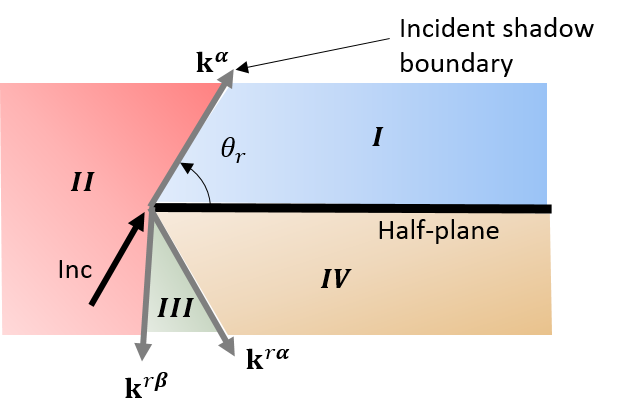
\includegraphics[height=0.33\textheight]{images/chapter1/ShadowBoundary.png}
    \caption{Incident wave on an edge}
    \label{illuzones}
\end{figure}

\subsection{\acrfull{gtd}}
\label{C1:GTD}
The \acrfull{gtd} was initially developed by Keller \cite{GTD} for optical waves and adapted to elastodynamics by Achenbach and Gautesen \cite{AchenbachGautesen, Achenbach}. This theory postulates the existence of diffracted waves emanating from the edge of the scattering surface. A incident ray on an edge generates a cone of rays, called Keller's cone of diffraction \cite{GTD}, represented on Fig.~\ref{KellerCone}. The cone's principal axis is the diffracting edge, its principal angle $\Omega_{\beta}$ is determined by Snell's law of diffraction :
\begin{equation}
    \frac{1}{c_{\alpha}}\cos\Omega_{\alpha} = \frac{1}{c_{\beta}} \cos\Omega_{\beta}
    \label{Snelldiff}
\end{equation}

\begin{figure}
    \centering
    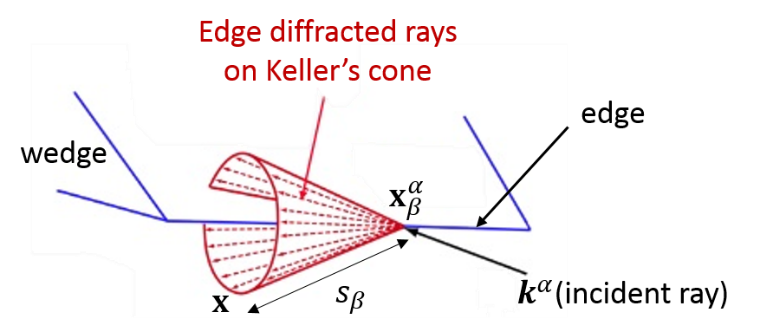
\includegraphics[width=\textwidth]{images/chapter1/KellerCone.png}
    \caption{Diffracted rays generated by an incident ray}
    \label{KellerCone}
\end{figure}
where $\Omega_{\alpha}$ is the angle between the incident wave vector and the diffracting edge. This cone has been observed by Rahmat-Samii \cite{ConePhoto} in a hotel room, see Fig.~\ref{PhotoCone}. A ray of light is incident on the corner of a table and generates a cone of diffracted rays, whose intersection with the door is a circle.

\begin{figure}
    \centering
    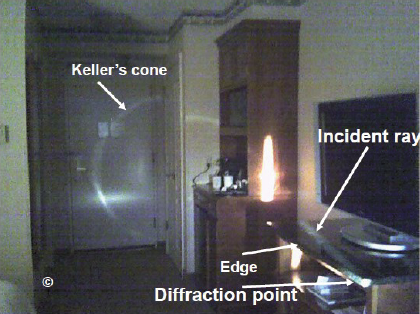
\includegraphics{images/chapter1/HotelCone.png}
    \caption{Observation of Keller's cone of diffraction}
    \label{PhotoCone}
\end{figure}

\acrshort{gtd} is also a ray tracing method, meaning that at a given observation point $\mathbf{x}$, the total field $\mathbf{u}^{tot}$ is the sum of the fields carried by each ray passing through $\mathbf{x}$ :
\begin{equation}
    \mathbf{u}^{tot}(\mathbf{x})=\mathbf{u}^{(GE)}(\mathbf{x})+\sum_{\beta} \mathbf{u}^{diff}_{\beta}(\mathbf{x})
    \label{GTDtot}
\end{equation}
where $\mathbf{u}^{(GE)}$ is the \acrshort{ge} displacement field, composed of the incident, reflected and refracted fields and $\mathbf{u}^{diff}_{\beta}$ is the diffracted field of type $\beta=L,TH,TV$. In this chapter, the bold font is used to denote vectors. The diffracted field's amplitude decreases as the distance $r$ from the point of impact $\mathbf{x}_{\beta}^{\alpha}$ of the incident wave on the diffracting edge grows. As for the \acrshort{ge} field, the diffracted field is proportional to the field incident on the edge. This proportionality is characterized by a multiplicative coefficient called the diffraction coefficient, which depends on the propagation medium, on the geometry of the diffracting object and on the direction of observation. This is summarized for an incident plane wave by the following equation :
\begin{equation}
    \mathbf{u}_{\beta}^{diff}(\mathbf{x})=u_{\alpha}(x_{\beta}^{\alpha})D_{\beta}^{\alpha}(\theta)\dfrac{e^{ik_{\beta}S_{\beta}}}{\sqrt{k_{\beta}r\sin\Omega_{\beta}}}\mathbf{e_{\beta}}(\mathbf{x})
    \label{C1:GTDdiff}
\end{equation}
where $u_{\alpha}$ is the scalar value of the incident field, $D_{\beta}^{\alpha}$ is the diffraction coefficient, $\theta$ is the direction of observation, $k_{\beta}$ is the diffracted wave's wave number, $S_{\beta}$ is the distance between the observation point $\mathbf{x}$ and the diffraction point $\mathbf{x}_{\beta}^{\alpha}$ (visible Fig.~\ref{KellerCone}) and $\mathbf{e_{\beta}}(M)$ is the unit polarization vector of the diffracted wave at point $\mathbf{x}$.

This principle is called the locality principle, because it stipulates that the value of the field at any given point is fully determined by the field in the close vicinity of the point from which the ray carrying this field emanates. Computation of diffracted fields can therefore be reduced to a number of canonical problems, such as diffraction by a tip or a half plane. In the present thesis, the canonical problem of interest is diffraction by a wedge.

\acrshort{gtd} is a high-frequency model which accounts for edge-diffracted waves. However, the resulting field is discontinuous at shadow boundaries and the diffraction coefficient possesses poles in the directions of geometrical reflection, rendering the diffracted field divergent in these directions. The resulting field is therefore not physical. Some uniform corrections have been proposed to solve this problem, resulting in continuous fields. They are presented in the following. 

\section{Uniform corrections}
\label{sectUnif}
\subsection{\acrfull{ka}}
\label{sectKA}
The \acrfull{ka}, also called \acrfull{po} was first developed in optics by Baker and Copson \cite{POoptics} before being extended to acoustic and electromagnetic waves \cite{POtechreport, POLewis} and being adapted by Chapman to elastic waves \cite{POChapman}, where it is essentially used for \acrshort{ndt} applications \cite{Schmerr,Dorval}.

The Kirchoff Approximation is a high frequency approximation for which the scattering surface is assumed to behave locally like a plane. This means that for each point of the surface, the plane tangent to the surface at that point is determined and the displacement field on the illuminated side is computed using \acrshort{ge}. The other side of the plane is shadowed and the total displacement field vanishes. The jump in the displacement between both sides of this plane is called \acrfull{cod} and noted $\lbrack \mathbf{u}(\mathbf{x}) \rbrack$. It leads to an integral formulation of the scattered field, called the Rayleigh-Sommerfeld integral \cite{POChapman} :
\begin{equation}
u_p(\mathbf{x})=\int_{S^+}\lbrack u_i(\mathbf{x'})\rbrack G_{ij}^{(p)}(\mathbf{x},\mathbf{x'})n_j(\mathbf{x'})\,d^2\mathbf{x'}
\label{intKA}
\end{equation}
where $u_p$ is the $p$-th coordinate of the displacement scattered field, $S^+$ is the lit side of the scattering surface, $n$ is the outward normal to $S^+$ and $G_{ij}^{(p)}(\mathbf{x},\mathbf{x'})$ is the $(ij)$ component of Green's stress tensor $G^{(p)}(\mathbf{x},\mathbf{x'})$, which is the stress produced at $\mathbf{x}$ by a unit traction acting along the $p$-axis at point $\mathbf{x'}$ on $S^+$, its expression is given in \cite{POChapman}. In this integral, Green's tensor is used to propagate the local solution $\lbrack \mathbf{u}(\mathbf{x'}) \rbrack$ to the whole propagation domain.

The \acrshort{ka} scattered field models diffraction and reflection and is continuous in the whole space. Comparisons between \acrshort{ka}, \acrshort{gtd} and the exact solution have been made for a strip-like crack illuminated by a transversal wave \cite{POChapman,systmodel}. \acrshort{ka} gives good results close to the geometrical reflections, as can be expected since the model is based on the \acrshort{ge} field. However, further away from these regions, it is inaccurate, as opposed to the \acrshort{gtd} which models diffraction correctly.

The \acrshort{gtd} solution, which models diffraction well, is non-uniform in the sense that it diverges at shadow boundaries. The \acrshort{ka} on the other hand, is uniform but doesn't model diffraction correctly. Furthermore, it requires meshing of the scattering surface. To overcome inaccuracies of the \acrshort{gtd} and \acrshort{ka} models, an other model has been developed, called the \acrfull{ptd}.

\subsection{\acrfull{ptd}}
The \acrfull{ptd} was first developed for acoustic and electromagnetic waves by Ufmitsev \cite{Ufmi} and was extended to elastodynamics in the case of a half-plane by Zernov et al. \cite{Zernov}. It is also applied to ultrasonic scattering near critical angles \cite{systmodel,FradkinDarmon}. The idea is to combine \acrshort{gtd} and \acrshort{ka} models to overcome their shortcomings. This is done by adding a corrective term to the \acrshort{ka} diffracted field which is the difference between the \acrshort{gtd} and the \acrshort{ka} diffracted fields :
\begin{equation}
\mathbf{u}^{tot (PTD)}=\mathbf{u}_{\alpha}(\mathbf{x})+\mathbf{u}^{sc (PTD)}(\mathbf{x})
\end{equation}
where $\mathbf{u}_{\alpha}$ is the incident field and
\begin{equation}
\mathbf{u}^{sc (PTD)}(\mathbf{x})=\sum_{\beta}\left[\mathbf{u}^{\alpha(KA)}_{\beta}(\mathbf{x})+u_{\alpha}(\mathbf{x}_{\beta}^{\alpha})\left(D_{\beta}^{\alpha(GTD)}(\mathbf{x})-D_{\beta}^{\alpha(KA)}(\mathbf{x})\right)\dfrac{e^{ik_{\beta}S_{\beta}}}{\sqrt{k_{\beta}r\sin\Omega_{\beta}}}\right]
\label{eqPTD}
\end{equation}
where  $\mathbf{u}^{\alpha(KA)}_{\beta}$ is obtained by \eqref{intKA}, $D_{\beta}^{\alpha(GTD)}$ is the \acrshort{gtd} diffraction coefficient and $D_{\beta}^{\alpha(KA)}$ is the \acrshort{ka} diffraction coefficient obtained by an asymptotic evaluation of \eqref{intKA} for $k_{\beta}S_{\beta}>>1$ (see appendix \ref{PhaseStationnaire}), which corresponds to the contribution of the scattering edges to the Rayleigh-Sommerfeld integral. In the far-field, the \acrshort{ka} diffraction coefficient diverges at specular directions, compensating the divergence of the \acrshort{gtd} diffraction coefficient. The diffracted field then disappears, leaving only the Kirchhoff evaluation, which is accurate in directions of geometrical reflection.

Far from the incident and specular directions, we have :
\begin{equation}
\mathbf{u}_{\beta}^{\alpha(KA)}(\mathbf{x})\approx \mathbf{u}_{\beta}^{diff(KA)}(\mathbf{x}) \approx u_{\alpha}(\mathbf{x}_{\beta}^{\alpha})D_{\beta}^{\alpha(KA)}(\mathbf{x})\dfrac{e^{ik_{\beta}S_{\beta}}}{\sqrt{k_{\beta}r\sin\Omega_{\beta}}}
\end{equation}
Substituting this into \eqref{eqPTD}, we find that in these regions, the \acrshort{ka} contribution vanishes and only the \acrshort{gtd} field remains, which models diffraction accurately.

The Physical theory of diffraction has been developed in the \acrshort{ndt} software platform CIVA \cite{systmodel}. It provides a good description of the scattered field in the directions of specular reflection, as well as far from the shadow boundaries. However, it requires meshing of the scattering surface for the \acrshort{ka} model as well as meshing of the flaw contour for the \acrshort{gtd} model, which can render it computationally expensive for large scatterers. Another uniform model has been developed, which does not required meshing of the scattering surface, called the \acrfull{uat}.

\subsection{\acrfull{uat}}
The \acrfull{uat} was first developed in for acoustics and electromagnetics by Lewis and Boersma \cite{Lewis} in two dimensions and was extended to three-dimensional problems by Ahluwalia \cite{Ahluwalia} and to a curved wedge by Lee and Deschamps \cite{LeeDeschamps} before being applied to elastodynamics by Achenbach et al. \cite{Achenbach}. It is a correction of the \acrshort{gtd} model where the \acrshort{ge} field is modified to compensate the divergence in the \acrshort{gtd} field and smooth the discontinuity in the \acrshort{ge} field. The total field \eqref{GTDtot} becomes :
\begin{equation}
\mathbf{u}^{tot(UAT)}(\mathbf{x})=\left[ \overline{F}(\xi_{\alpha})-\hat{\overline{F}}(\xi_{\alpha})\right]\mathbf{u}_{\alpha}(\mathbf{x})+\sum_{\beta} \left[ \overline{F}(\xi_{\beta})-\hat{\overline{F}}(\xi_{\beta})\right]\mathbf{u}^{ref}_{\beta}(\mathbf{x})+\mathbf{u}_{\beta}^{diff(GTD)}(\mathbf{x})
\label{eqUAT}
\end{equation}
where $\overline{F}$ is the Fresnel function, defined by 
\begin{equation}
\overline{F}(X)=\frac{1}{\sqrt{i\pi}}\int_X^{+\infty} e^{it^2}\,dt
\label{defFresnel}
\end{equation}
and 
\begin{equation}
\hat{\overline{F}}(X)=e^{i\frac{\pi}{4}}\dfrac{e^{iX^2}}{2X\sqrt{\pi}}
\end{equation}
$\mathbf{u}^{ref}_{\beta}$ is the reflected field of type $\beta$, $\mathbf{u}_{\beta}^{diff(GTD)}$ is the \acrshort{gtd} diffracted field of type $\beta$ and $\xi_{\alpha}$ and $\xi_{\beta}$ are detour parameters defined in \cite{LeeDeschamps}. They evaluate the proximity of the observation point to the shadow boundary of the incident wave for $\xi_{\alpha}$ and of the reflected wave for $\xi_{\beta}$. The presence of the Fresnel function $\overline{F}$ smooths the discontinuity in the \acrshort{ge} field while the function $\hat{\overline{F}}$ compensates the divergence of the \acrshort{gtd} diffracted field. Therefore, the total \acrshort{uat} field is spatially uniform. Note that in \eqref{eqUAT} the incident and reflected fields are defined in the the whole space. This means in particular that they must be extended to their shadow zones. This is achieved by constructing the fictitious rays in the shadow zones \cite{Bouche,Molinet}, see Fig.~\ref{FictRays}. 

\acrshort{uat} is a spatially uniform method which models diffraction accurately. However, it requires tracing of fictitious rays and is therefore difficult to implement for complex geometries. To overcome this difficulty, a uniform model which is simpler to implement, the \acrfull{utd} has been developed.

\begin{figure}[h]
    \centering
    \begin{subfigure}[b]{0.45\textwidth}
        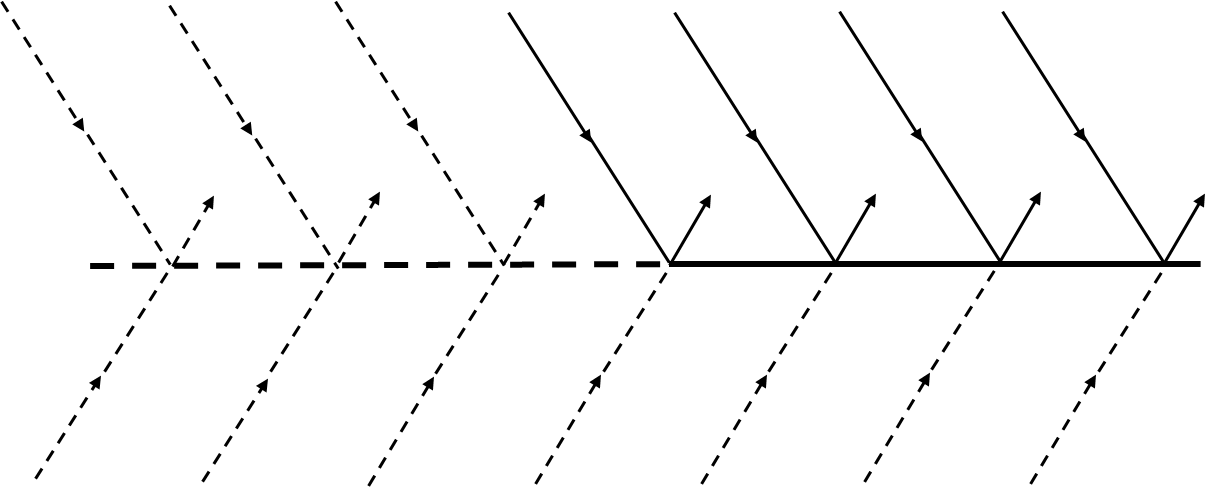
\includegraphics[width=\textwidth]{images/chapter1/FictitiousStraight.png}
        \caption{Fictitious rays constructed in the case of a straight scatterer}
        \label{Straightfict}
    \end{subfigure}
    ~ 
    \begin{subfigure}[b]{0.45\textwidth}
        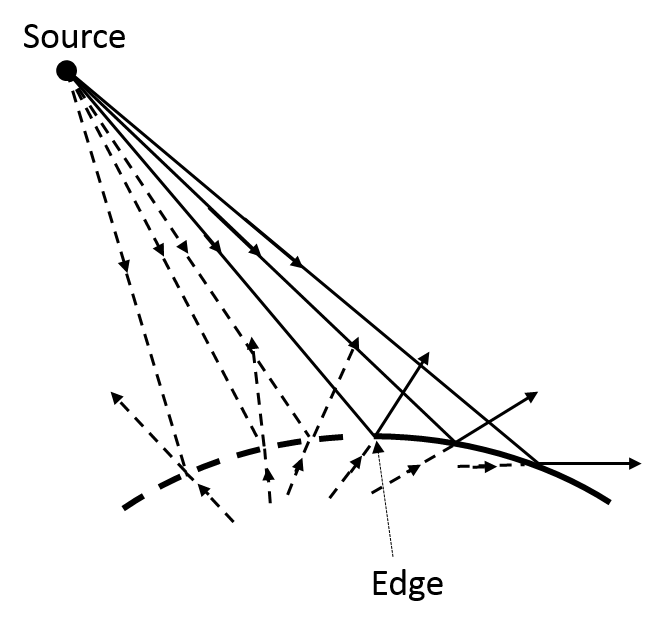
\includegraphics[width=\textwidth]{images/chapter1/FictitiousCurved.png}
        \caption{Fictitious rays constructed in the case of a curved scatterer}
        \label{Curvedfict}
    \end{subfigure}
    \caption{(Reproduced from \cite{Bouche,Molinet}) Extension of the reflected field to its shadow zone using fictitious rays. Dashed thick lines are extensions of the scatterers beyond the crack edge and dashed thin lines are incident and fictitious reflected rays on these extensions.}
    \label{FictRays}
\end{figure}

\subsection{\acrfull{utd}}
The \acrfull{utd} was initially developed for acoustic and electromagnetic waves by Kouyoumjian and Pathak \cite{Kouyoumjian,PathakKouyou} and was extended to elastodynamics by Kamta-Djakou during her PhD thesis \cite{Audrey,AKDthese}. This method consists of correcting the \acrshort{gtd} diffraction coefficient using a transition function $F$. For the problem of diffraction by a wedge of angle $\varphi$, this is expressed as :
\begin{equation}
    D_{\beta}^{\alpha(UTD)}(\zeta,\theta)=(-1)^{M_{\beta}+1}D_{\beta}^{\alpha(GTD)}(\theta)\left[ \sum_{j=1}^{M_{\beta}} F(\zeta a^j_{\beta})\prod_{\underset{k\neq j}{k=1}}^{M_{\beta}} \dfrac{s_\beta^{k}}{(s_\beta^{j}-s_\beta^{k})}\right]
    \label{DUTDGTD}
\end{equation}
where $\theta$ is the direction of observation, $(\lambda^j_{\beta}), 1\leq j\leq M_{\beta}$ are the poles of the diffraction coefficient mentioned in section \ref{C1:GTD} (methods of computation of these poles will be given in the following chapters) and 
\begin{equation}
    a_{\beta}^j=-i(s_{\beta}^j)^2=2\cos^2\left(\frac{\lambda_{\beta}^j-\theta+\varphi/2}{2}\right)
\end{equation}
$\zeta$ is a far-field parameter which can be defined as
\begin{equation}
    \zeta=k_{\beta}r\sin\Omega_{\beta}.
\end{equation}
Finally, $F$ is a transition function defined as the complex conjugate of the Kouyoumjian function \cite{Kouyoumjian}
\begin{equation}
    F(X)=-2i\sqrt{i\pi X}e^{-iX}\overline{F}(\sqrt{X})
\end{equation}
$\overline{F}$ is the Fresnel function defined by \eqref{defFresnel}.

Far from the shadow boundaries, $\zeta a_{\beta}^j >>1$ and
\begin{equation}
F(\zeta a_{\beta}^j) \rightarrow 1 \mbox{ and } (-1)^{M_{\beta}+1}\left[ \sum_{j=1}^{M_{\beta}} \prod_{\underset{k\neq j}{k=1}}^{M_{\beta}} \dfrac{s_\beta^{k}}{(s_\beta^{j}-s_\beta^{k})}\right]=1
\end{equation}
In this case, the \acrshort{utd} solution for the diffracted field is the same as the \acrshort{gtd} diffracted field. Close to the shadow boundaries, Kamta-Djakou \cite{AKDthese} has shown that the transition functions makes the diffracted field discontinuous when crossing shadow boundaries and that these irregularities compensate exactly those of the \acrshort{ge} field, so that the total field computed using \eqref{GTDtot} is uniform.

The \acrfull{utd} has been validated numerically in far-field configurations in \cite{AKDthese}. It models the diffracted field well and provides a spatially uniform solution while being simple to implement.

The \acrshort{ptd}, \acrshort{uat} and \acrshort{utd} methods presented are all uniform \textit{corrections} of the \acrshort{gtd} field. This means that they all rely on a preexisting \acrshort{gtd} solution, which must therefore be accurate. In the following, the two main existing \acrshort{gtd} approaches to the problem of diffraction of an elastic wave by a stress-free wedge are presented.

\section{Principal \acrshort{gtd} elastic wedge diffraction models}

\begin{figure}
\centering
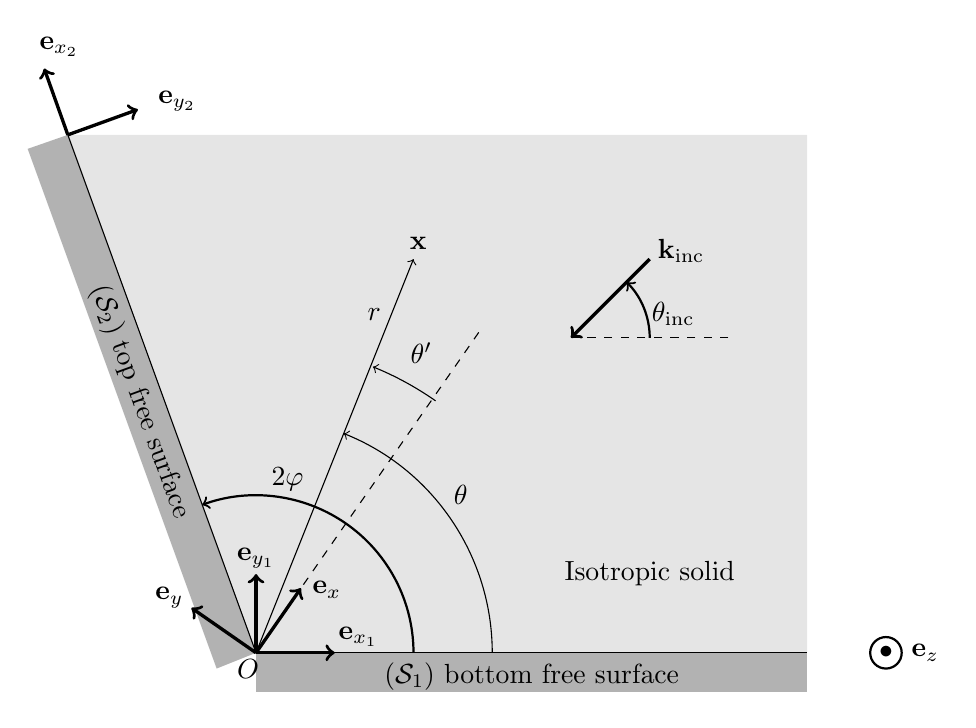
\begin{tikzpicture}
\fill[color=gray!20] (0,0) -- (7,0)  -- (7,6.5778) -- (-2.39,6.5778) -- cycle;  
\draw[ thick, ->] (2,0) arc (0:110:2);

\fill[color=gray!60] (0,0) -- (7,0)  -- (7,-0.5) -- (0,-0.5) -- cycle;  

\fill[color=gray!60] (0,0) --  (-2.39,6.5778) --(-2.9,6.4) -- (-0.5,-0.2) -- cycle; 

\draw[color = black]  (0,0) -- (7,0) node[midway,below] {($\mathcal{S}_1$) bottom free surface};

\draw[color = black]  (0,0) -- (-2.39,6.5778) node[midway,below,sloped] { ($\mathcal{S}_2$) top free surface};

\draw[very thick, ->] (-2.39,6.5778) -- (-2.69,7.42);

\node[scale=1] at (-2.5,7.7){ $\mathbf{e}_{x_2}$};

\draw[very thick, ->] (-2.39,6.5778) -- (-1.5,6.9);

\node at (-1,7){$\mathbf{e}_{y_2} $};


\node at (0.4,2.2){$2 \varphi$} ; 

\draw[very thick, ->] (0,0) -- (1,0);

\node at (1.3,0.2) {$\mathbf{e}_{x_1} $};

\draw[very thick, ->] (0,0) -- (0,1);

\node at (0,1.2){$\mathbf{e}_{y_1} $};

\node at (8,0) {$\bullet$};

\draw[thick] (8,0) circle (0.2);

\node at (8.5,0){$\mathbf{e}_{z}$};

\draw[very thick, ->] (0,0) -- (0.57,0.82);

\node at (0.9,0.8){$\mathbf{e}_x$};

\draw[very thick, ->] (0,0) -- (-0.82, 0.57);

\node at (-1.1,0.7){$\mathbf{e}_y$};

\draw[very thick, ->] (5,5) -- (4,4);

\draw[dashed] (6,4) -- (4,4);

\draw[ thick, ->] (5,4) arc (0:45:1);

\node at (5.3,4.3){$\theta_{\rm inc}$};

\node at (5.4,5.1){$\mathbf{k}_{\rm inc}$};

\node at (-0.1,-0.2){$O$};

\node at (5,1){Isotropic solid};

% point observation

\draw[->] (0,0) -- (2,5); 

\draw[->] (3,0) arc (0:68.2:3);

\draw[dashed] (0,0) -- (2.85,4.1);

\node at (2.6,2){$\theta$};

\node at (1.5,4.3){$r$};

\node at (2.06,5.2){$\mathbf{x}$};

\draw[->] (2.28,3.2) arc (55:68:4);

\node at (2.1,3.8){$\theta'$};

\end{tikzpicture}
\caption{Stress-free wedge of angle $2\varphi$ illuminated by a plane wave of wave vector $\mathbf{k}^{\rm inc}$. The dotted line is the wedge bisector.}
\label{C1:wedge}
\end{figure}

As seen in the previous section, an accurate uniform scattering model requires a trust-worthy initial \acrshort{gtd} solution in order to be developed. The aim of this thesis will therefore be to develop a generic and trust-worthy wedge diffraction \acrshort{gtd} model. To our knowledge, there is no fully analytical resolution of the problem of elastic wedge diffraction available in scientific literature, and the preferred approach is semi-analytical. We begin this work by a review of the two main existing 2D elastic wedge-diffraction models. These two models have been presented and compared by Gautesen and Fradkin \cite{GautesenFradkin}, who also discuss their numerical validation. Experimental validation  of these codes has been done by Chapman et al. \cite{ChapmanLTval}.

\subsection{Problem statement}
\label{C1:PbStatement}
The geometry of the problem is visible in Fig.~\ref{C1:wedge}. A stress-free wedge of angle $2\varphi<\pi$ is illuminated by a a plane wave which forms an angle $\theta_{inc}$ with the bottom face of the wedge. The problem is two-dimensional in the sense that the incident wave vector is in the plane normal to wedge edge. In all the following, the harmonic time-dependency factor $e^{- i\omega t}$ (where $\omega$ is the circular frequency and $t$ is time) will be omitted. $(0;\mathbf{e}_{x_1},\mathbf{e}_{y_1},\mathbf{e}_z)$ is the orthonormal basis of a Cartesian coordinate system where the $z$-axis coincides with the wedge edge and the $x_1$ axis coincides with the bottom face of the wedge. The polar coordinates associated to this system are $\mathbf{x}=(r,\theta)$. In this coordinate system, the incident wave vector is :
\begin{equation}
\mathbf{k}^{inc}=-(\cos\theta_{inc},\sin\theta_{inc})_{(\mathbf{e}_{x_1},\mathbf{e}_{y_1})}
\end{equation}
$(0;\mathbf{e}_x,\mathbf{e}_y,\mathbf{e}_z)$ is the orthonormal basis of a Cartesian coordinate system where the $x$-axis coincides with the wedge bisector and the polar coordinates associated to the system are $\mathbf{x}=(r,\theta')$.

In both of the following approaches, the the symmetry of the problem with respect to the wedge bisector is used and the problem is split in two : a symmetric problem, regarding the polarization of the incident wave, and an antisymmetric problem. This is done by introducing a wave vector symmetric to $\mathbf{k}^{inc}$ with respect to the bisector :
\begin{equation}
\mathbf{k}_{sym}=(-\cos\theta'_{inc},\sin\theta'_{inc})_{(\mathbf{e}_x,\mathbf{e}_y)}
\end{equation}
In the case of an incident L wave, the symmetric problem is constructed by considering that the incident wave is the sum of two plane waves of which the wave vectors are $\mathbf{k}^{inc}$ and $\mathbf{k}_{sym}$, see Fig.~\ref{Sym}. In this case, the polarization vectors $\mathbf{p}^{inc}=\mathbf{k}^{inc}$ and $\mathbf{p}_{sym}=\mathbf{k}_{sym}$ are symmetric. The antisymmetric problem is constructed by setting the incident wave to be the sum of two plane waves of which the wave vectors are $\mathbf{k}^{inc}$ and $-\mathbf{k}_{sym}$, see Fig.~\ref{Antisym}. In this case the polarization vectors $\mathbf{p}^{inc}$ and $-\mathbf{p}_{sym}$ are antisymmetric.

In the case of an incident T wave, the polarization vector is normal to the wave vector. Therefore, symmetric problem is constructed by setting $\mathbf{k}^{inc}$ and $-\mathbf{k}_{sym}$ as the incident wave vectors, see Fig.~\ref{Antisym} and the antisymmetric problem is constructed by setting $\mathbf{k}^{inc}$ and $\mathbf{k}_{sym}$ as the incident wave vectors, see Fig.~\ref{Sym}.

\begin{figure}[h]
    \centering
    \begin{subfigure}[b]{0.45\textwidth}
        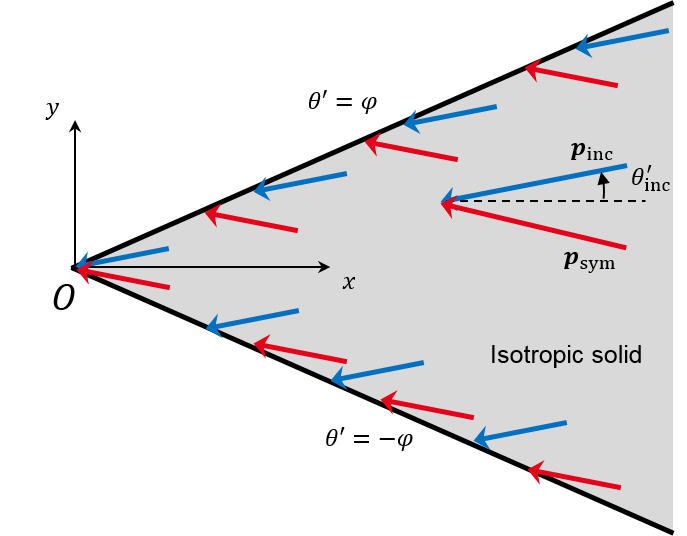
\includegraphics[width=\textwidth]{images/chapter1/SymPb.png}
        \caption{Symmetric problem for an incident longitudinal wave or antisymmetric problem for an incident transversal wave}
        \label{Sym}
    \end{subfigure}
    ~ 
    \begin{subfigure}[b]{0.45\textwidth}
        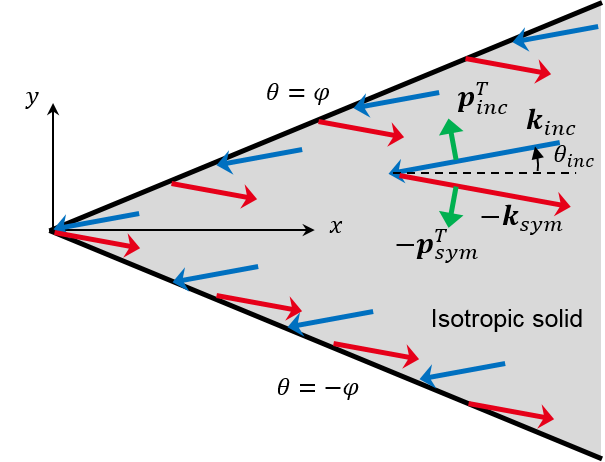
\includegraphics[width=\textwidth]{images/chapter1/AntisymPb.png}
        \caption{Antisymmetric problem for an incident longitudinal wave or symmetric problem for an incident transversal wave}
        \label{Antisym}
    \end{subfigure}
    \caption{Symmetric and antisymmetric problems. Blue and red vectors are the wave vectors and green vectors are the polarization vectors of the transversal waves.}
    \label{SymAntisym}
\end{figure}

Both of the semi-analytic resolutions that will be described in the following deal with the symmetric and antisymmetric problems separately, in order to reduce the numerical part of the resolution by half. The first approach presented is called the \acrfull{si} method. The main steps of the resolution are presented but the technical details are not given.

\subsection{The \acrfull{si} Method}
The \acrfull{si} method was first proposed by Budaev \cite{BudaevBook,Budaev1,Budaev2} and Budaev and Bogy \cite{Rayleigh,Rayleigh2,Rayleigh3} have proposed the corresponding numerical scheme. The theory was completed and clarified by Kamotski et al. \cite{KamotskiFradkin}.

In this approach, the elastodynamic potentials $\psi_L$ and $\psi_T$ are the unknowns. They are related to the displacement field by :
\begin{equation}
\mathbf{u}=\mathbf{\nabla}\psi_L+\mathbf{\nabla}\times(\psi_T\mathbf{e}_z)
\label{C1:elastopotentials}
\end{equation}
where $\mathbf{\nabla}$ is the gradient operator and $\mathbf{\nabla}\times$ is the curl operator. These potentials satisfy the Helmoltz equations in the angular domain \cite{Achenbach} :
\begin{equation}
\Delta \psi_L+k_L^2\psi_L=0 \mbox{ and } \Delta \psi_T+k_T^2\psi_T=0 \rm \mbox{ for } |\theta'|<\varphi
\label{C1:Helmoltz}
\end{equation}
In addition, the wedge faces are stress-free, meaning :
\begin{equation}
\sigma_{r\theta'}=0 \mbox{ and } \sigma_{\theta'\theta'}=0 \mbox{ for } |\theta'|=\varphi
\label{C1:stresses}
\end{equation}
Sommerfeld \cite{Sommerfeld} has given an exact expression of these potentials in the form of an integral. This integral satisfies \eqref{C1:Helmoltz} as well as the radiation conditions at infinity \cite{SMtechnique} :
\begin{equation}
\psi_*(k_*r,\theta')=\int_{\gamma_++\gamma_-}e^{-ik_*r\cos\lambda}\Psi_*(\theta'+\lambda)\,d\lambda
\label{C1:Sommerfeld}
\end{equation}
where $*=L,T$,$\lambda$ is a complex angle, $\Psi_*$ are unknown amplitudes and contours $\gamma_+$ and $\gamma_-$ are represented on Fig.~\ref{C1:Somcontours}.

\begin{figure}
\centering
\begin{tikzpicture}
\fill[color=gray!20] (0,0) -- (0,3.5)  -- (pi,3.5) -- (pi,0);
\fill[color=gray!20] (-pi,-3.5) -- (0,-3.5)  -- (0,0) -- (-pi,0);
\fill[color=gray!20] (pi,-3.5) -- (4.5,-3.5)  -- (4.5,0) -- (pi,0);
\fill[color=gray!20] (-4.5,0) -- (-pi,0)  -- (-pi,3.6) -- (-4.5,3.6);
\draw[thin] (-4.5,0)  -- (4.5,0) node[above]{$\sigma$};
\draw[thin](0,-3.5)--(0,3.5) node[left]{$\tau$};
\draw[thin] (-pi,-3.5)  -- (-pi,3.5);
\draw[thin] (pi,-3.5)  -- (pi,3.5);
\node at (-3.4,-0.2) {$-\pi$};
\node at (3.3,0.2) {$\pi$};
\node at (-0.2,0.2) {$0$};
\node at (-2,1.0) {$\gamma_+$};
\node at (2,-1.0) {$\gamma_-$};

% segment de branche de coupure
%\draw[very thick] (-4, 0) -- (-2.2, 0);
%\draw[very thick] (4, 0) -- (2.2, 0);
%\draw (-4, 0) node {$\bullet$} ;
%\draw (-2.2, 0) node {$\bullet$} ;
%\draw (4, 0) node {$\bullet$} ;
%\draw (2.2, 0) node {$\bullet$} ;

% sommerfeld contour -pi
%\draw[black,very thick][domain=0:4.8] plot({-pi - acos(1/cosh(\x))*pi/180},\x);
%\draw[black,very thick][domain=-4.8:0] plot({-pi + acos(1/cosh(\x))*pi/180},\x);

% \draw[very thick,black,
%decoration={ markings,  % This schema allows for fine-tuning the positions of arrows 
%      mark=at position 0.1 with {\arrow{latex}}},
%      postaction={decorate}]
%      (-2.6404,-pi/6)  -- (-3.6428,pi/6); 

% sommerfeld contour pi
%\draw[black,very thick][domain=0:4.8] plot({pi - acos(1/cosh(\x))*pi/180},\x);
%\draw[black,very thick][domain=-4.8:0] plot({pi + acos(1/cosh(\x))*pi/180},\x);

% \draw[very thick,black,
%decoration={ markings,  % This schema allows for fine-tuning the positions of arrows 
%      mark=at position 0.1 with {\arrow{latex}}},
%      postaction={decorate}]
%     (2.6404,pi/6) -- (3.6428,-pi/6); 

% sommerfeld contour 0
%\draw[black,very thick, dashed][domain=0:4.8] plot({0 + acos(1/cosh(\x))*pi/180},\x);
%\draw[black,very thick, dashed][domain=-4.8:0] plot({0 - acos(1/cosh(\x))*pi/180},\x);

% \draw[thick,dashed,
%decoration={ markings,  % This schema allows for fine-tuning the positions of arrows 
%      mark=at position 0.1 with {\arrow{latex}}},
%      postaction={decorate}]
%      ( -0.5012,-pi/6)  -- (0.5012,pi/6); 

\draw[very thick,black,xshift=0pt,
decoration={ markings,  % This schema allows for fine-tuning the positions of arrows 
      mark=at position 0.2 with {\arrow{latex}},
      mark=at position 0.5 with {\arrow{latex}},
      mark=at position 0.9 with {\arrow{latex}}},
      postaction={decorate}]
      (0.2,3.5) -- (0.2,0.8) -- (-pi-0.2,0.8) -- (-pi -0.2,3.5); 
      
\draw[very thick,black,xshift=0pt,
decoration={ markings,  % This schema allows for fine-tuning the positions of arrows 
      mark=at position 0.2 with {\arrow{latex}},
      mark=at position 0.5 with {\arrow{latex}},
      mark=at position 0.9 with {\arrow{latex}}},
      postaction={decorate}]
      (-0.2,-3.5) -- (-0.2,-0.8) -- (pi+0.2,-0.8) -- (pi +0.2,-3.5);
\end{tikzpicture}
\caption{Sommerfeld contours of integration $\gamma_+$ and $\gamma_-$ in the complex plane $\lambda=\sigma+i\tau$.}
\label{C1:Somcontours}
\end{figure}

Following the decomposition of the problem, the unknown amplitudes can be decomposed into symmetric and antisymmetric amplitudes. The superscript $"+"$ refers to the symmetric problem and the superscript $"-"$ refers to the antisymmetric one. We then have :
\begin{equation}
\Psi_*(\lambda)=\Psi_*^+(\lambda)+\Psi_*^-(\lambda)
\end{equation}
where
\begin{subequations}
\begin{equation}
\Psi_L^\pm(\lambda)=\frac{1}{2}\lbrack\Psi_L(\lambda)\pm\Psi_L(-\lambda)\rbrack
\end{equation}
\begin{equation}
\Psi_T^\pm(\lambda)=\frac{1}{2}\lbrack\Psi_L(\lambda)\mp\Psi_L(-\lambda)\rbrack
\end{equation}
\end{subequations}
The symmetric and antisymmetric potentials $\psi_*^\pm$ associated to these amplitudes using \eqref{C1:Sommerfeld} are the solutions of the symmetric and antisymmetric problems. Kamotski et al. \cite{KamotskiFradkin} have shown that subsituting \eqref{C1:Sommerfeld} into \eqref{C1:stresses} yields the following system of functional equations :
\begin{multline}
\begin{pmatrix}
\Psi_L^\pm(g(\lambda)+\varphi)\\
\Psi_T^\pm(\lambda+\varphi)
\end{pmatrix}
=\pm\begin{pmatrix}
r_L^L(\lambda)&r_L^T(\lambda)\\
r_T^L(\lambda)&r_T^T(\lambda)
\end{pmatrix} 
\begin{pmatrix}
\Psi_L^\pm(g(\lambda)-\varphi)\\
\Psi_T^\pm(\lambda-\varphi)
\end{pmatrix} \\
+\kappa^2 c_1^\pm\dfrac{\sqrt{\kappa^{-2}-\cos^2\lambda}}{\mathcal{R}(\lambda)} \begin{pmatrix}
\cos 2\lambda-\tan\varphi\sin 2\lambda \\
\sin 2\lambda+\tan\varphi\dfrac{\sin\lambda\cos 2\lambda}{\sqrt{\kappa^{-2}-\cos^2\lambda}}
\end{pmatrix}
\label{C1:SIfunctional}
\end{multline}
where $\kappa=c_L/c_T$,
\begin{equation}
g(\lambda)=\arccos(\kappa\cos\lambda),
\end{equation}
the potential reflection coefficients $r_L^L,r_L^T,r_T^L$ and $r_T^T$ for the traction-free elastic half-space are known explicitly and are given in \cite{KamotskiFradkin}, function $\mathcal{R}$ is called the Rayleigh function :
\begin{equation}
\mathcal{R}(\lambda)=\cos^2 2\lambda+2\sqrt{\kappa^{-2}-\cos^2\lambda}\sin 2\lambda \cos\lambda
\label{C1:defRayleigh}
\end{equation}
and finally $c_1^\pm$ are unknown constants.

Representation \eqref{C1:Sommerfeld} gives the total elastodynamic potentials, including incident and reflected fields. It is well known that the poles of the Sommerfeld amplitudes $\Psi_*$ lead to the \acrshort{ge} field. The Sommerfeld amplitudes $\Psi_*^\pm$ can therefore be decomposed into two parts : a "singular part" $\Psi_*^{\pm \, sing}$, containing these poles and a "regular part" $\Psi_*^{\pm \, reg}$
\begin{equation}
\Psi_*^\pm=\Psi_*^{\pm \, sing}+\Psi_*^{\pm \, reg}
\label{C1:singreg}
\end{equation}
where $\Psi_*^{\pm \, reg}$ is regular in the strip 
\begin{equation}
\{ \lambda \in \mathbb{C},\, \pi/2-\varphi \leq \rm Re \lambda \leq \pi/2+\varphi \}
\end{equation}
and
\begin{equation}
\Psi_*^{\pm sing}(\lambda)=\sum_j \dfrac{res^\pm(\pm \lambda_*^j)}{2}\cot\left(\dfrac{\lambda\mp\lambda_*^j}{2}\right)
\end{equation}
$\pm\lambda_*^j$ are the poles of the Sommerfeld amplitudes $\Psi_*^{\pm sing}$ and  $res^\pm(\pm \lambda_*^j)$ are the corresponding residues. These poles and residues are determined analytically thanks to a recursive pole propagation algorithm, which is explained in great detail by Kamta-Djakou in \cite{AKDthese} and will not be reproduced here. Decomposition \eqref{C1:singreg} is then substituted into \eqref{C1:SIfunctional} and the resulting system is solved numerically, thanks to the scheme proposed by Kamotski et al. \cite{KamotskiFradkin}.

The diffracted elastodynamic potentials $\psi_{\beta}^{GTD} $ can be expressed in terms of the Sommerfeld amplitudes by evaluating integral \eqref{C1:Sommerfeld} asymptotically with the steepest descent method (see appendix \ref{PhaseStationnaire}) :
\begin{equation}
\psi_{\beta}^{GTD}=(k_{\beta} r,\theta')=i\sqrt{2i\pi}\lbrack \Psi_{\beta}(\theta'-\pi)-\Psi_{\beta}(\pi+\theta')\rbrack \dfrac{e^{ik_{\beta}r}}{\sqrt{k_{\beta}r}}
\end{equation}
Using \eqref{C1:elastopotentials}, the diffracted displacement field are given by :
\begin{equation}
\mathbf{u}_{\beta}^{diff(SI)}(r,\theta')=D_L^{SI}(\theta')\dfrac{e^{ik_Lr}}{\sqrt{k_Lr}}\mathbf{e}_{r'}+D_T^{SI}(\theta')\dfrac{e^{ik_Tr}}{\sqrt{k_Tr}}\mathbf{e}_{\theta'}
\end{equation}
where
\begin{equation}
D_{\beta}^{SI}=-k_{\beta}\sqrt{2i\pi}\lbrack \Psi_{\beta}(\theta'-\pi)-\Psi_{\beta}(\pi+\theta')\rbrack
\end{equation}

To summarize, following the steps of Kamotski et al. \cite{KamotskiFradkin}, the \acrshort{gtd} diffraction coefficient of a stress-free wedge of angle $2\varphi<\pi$ can be computed. First, Sommerfeld's integral formulation of the elastodynamic potentials \eqref{C1:Sommerfeld} is used to determine two systems (one for the symmetric problem and once for the antisymmetric problem) of functional equations \eqref{C1:SIfunctional} of which the symmetric and antisymmetric Sommerfeld amplitudes are solution. These systems are then solved by determining the poles and residues of the Sommerfeld amplitudes analytically and computing the remaining regular function numerically. Finally, the \acrshort{gtd} diffraction coefficient is deduced. 

An other semi-analytic resolution technique is called the \acrfull{lt} method and is presented in the following. Once again, the main steps of the resolution will be presented but the technical details are not given.

\subsection{The \acrfull{lt} Method}
The \acrfull{lt} method is due to Gautesen, who had developed it in the case of an incident Rayleigh wave \cite{GautesenRayleigh,GautesenRayleigh2,GautesenRayleigh0,GautesenRayleigh3,GautesenRayleigh4}, and in the case of an incident longitudinal wave on a right-angled wedge\cite{GautesenLwave}. It has been extended to the case of an L or T elastic wave incident on a wedge of angle $2\varphi<\pi$ by Gautesen and Fradkin \cite{GautesenFradkin}.

In this approach, the unknown quantity is the elastodynamic displacement $\mathbf{u}=(u_1,u_2)_{(\mathbf{e}_{x_1},\mathbf{e}_{y_1})}$. Gautesen \cite{GautesenRayleigh} has expressed the components of the displacement field in the entire space (not just inside the wedge) as a single-layer potential, analogously to Lax's electromagnetic extinction theorem \cite{Lax} :
\begin{multline}
H(2\varphi-\theta)u_p(\mathbf{x})=u_p^{inc}(\mathbf{x})-\sum_{i=1}^2\int_0^{+\infty}\Big[ G_{i2}^{(p)}(x_1-l,x_2)u_i(l,0) \\
 +\sum_{j=1}^2\sum_{m=1}^2\sigma_{jm}^{(p)}(x_1-l\cos 2\varphi,x_2-l\sin 2\varphi)e_{x_2}^{(j)}e_{y_2}^{(m)}u^{(i)}(l) \Big] \, dl
 \label{C1:extthm}
\end{multline}
where $(0;\mathbf{e}_{x_2},\mathbf{e}_{y_2}, \mathbf{e}_z)$ is an orthonormal basis, shown on Fig.~\ref{C1:wedge} where the $x_2$-axis coincides with the top free surface and where $\mathbf{e}_{y_2}$ is directed towards the inside of the wedge, $G^{(p)}$ is Green's stress tensor, defined in section \ref{sectKA} and
\begin{eqnarray}
u^{(i)}(l)=
\left\{
\begin{array}{cc}
\mathbf{u}(l\cos 2\varphi,l\sin 2\varphi).\mathbf{e}_{x_2} & \mbox{ for } i=1 \\
\mathbf{u}(l\cos 2\varphi,l\sin 2\varphi).\mathbf{e}_{y_2} & \mbox{ for } i=2
\end{array}
\right.
\end{eqnarray}
Equation \eqref{C1:extthm} is simplified by working in the region $x_2<0$ where, in the case $2\varphi<\pi$, the left-hand side of \eqref{C1:extthm} vanishes. The equation then contains four unknowns $(u_1,u_2)(l,0)$ and $(u^{(1)},u^{(2)})(l)$. In order to reduce the number of unknowns by half, the problem is once again symmetrized as described in subsection \ref{C1:PbStatement}. As in the previous section, the $"+"$ sign describes the symmetric problem and the $"-"$ sign describes the antisymmetric problem. We then have :
\begin{equation}
u^{(i)\pm}(l)=\pm u_i^\pm(l,0), \hspace{2em} i=1,2, \hspace{2em} l>0
\end{equation}
Equation \eqref{C1:PbStatement} is then reduced to :
\begin{multline}
u_p^{inc \pm}(\mathbf{x})=\sum_{i=1}^2\int_0^{+\infty}\Big[ G_{i2}^{(p)}(x_1-l,x_2)u_i^\pm(l,0)\\
\pm\sum_{j=1}^2\sum_{m=1}^2\sigma_{jm}^{(p)}(x_1-l\cos 2\varphi,x_2-l\sin 2\varphi)e_{x_2}^{(j)}e_{y_2}^{(m)}u_i^\pm(l,0) \Big] \, dl
\label{C1:extthmsym}
\end{multline}
The Laplace transform of the displacement field is defined by :
\begin{equation}
\hat{u}_i(\xi)=k_T\int_0^{+\infty}u_i^\pm(l,0)e^{ik_Tl\xi}\, dl
\label{C1:defLapl}
\end{equation}
In the Laplace domain, for the sake of simplicity, the superscript $\pm$ is omitted but implied. In order to separate the contributions of the longitudinal and transversal waves, the curl and divergence operators of equation \eqref{C1:extthmsym} are successively taken. The Laplace transform, defined by \eqref{C1:defLapl}, is then applied to the resulting system, yielding
\begin{equation}
A(\xi)\begin{pmatrix}
\hat{u}_1(\xi)\\
\hat{u}_2(\xi)
\end{pmatrix}
= \begin{pmatrix}
f_T(\xi)-\hat{U}_Ts(\xi)\\
f_L(\xi)-\hat{U}_L(\xi)
\end{pmatrix}
\label{C1:LTsyst}
\end{equation}
where $U_T=\mathbf{\nabla}\times\mathbf{u}^\pm$ and $U_L=\mathbf{\nabla}.\mathbf{u}^\pm$ and 
\begin{subequations}
\begin{equation}
\hat{U}_T(\xi)=\pm\lbrack -a(T_T)\hat{u}_1(T_T)+\overline{b}_T(\xi)\hat{u}_2(T_T) \rbrack
\end{equation}
\begin{equation}
\hat{U}_L(\xi)=\pm\lbrack \overline{b}_L(\xi)\hat{u}_1(T_L)+a(T_L)\hat{u}_2(T_L) \rbrack
\end{equation}
\label{C1:ULUT}
\end{subequations}
and
\begin{equation}
A(\xi)=\begin{pmatrix}
a(\xi)&-b_T(\xi)\\
b_L(\xi)&a(\xi)
\end{pmatrix}
\label{C1:matA}
\end{equation}
In equations \eqref{C1:ULUT} and \eqref{C1:matA}, we have, for $*=L,T$ :
\begin{subequations}
\begin{equation}
a(\xi)=\kappa_T-2\xi^2
\end{equation}
\begin{equation}
b_*(\xi)=2\xi\gamma_*(\xi)
\end{equation}
\begin{equation}
\overline{b}_*(\xi)=2T_*\eta_*
\end{equation}
\end{subequations}
where $\kappa_*=c_L/c_*$ and
\begin{subequations}
\begin{equation}
\gamma_*(\xi)=\sqrt{\kappa_*^2-\xi^2}
\end{equation}
\begin{equation}
T_*(\xi)=\xi\cos 2\varphi+\gamma_*(\xi)\sin 2\varphi
\end{equation}
\begin{equation}
\eta_*(\xi)=\xi\sin 2\varphi-\gamma_*(\xi)\sin 2\varphi
\end{equation}
\end{subequations}
and finally
\begin{eqnarray}
f_*(\xi)=\left\{
\begin{array}{cc}
\mp2\pi\kappa_*^2\lbrack \sin\theta_{inc}\delta(\xi-\kappa_*\cos\theta_{inc})\sin(2\varphi-\theta_{inc})\delta(\xi-\kappa_*\cos(2\varphi-\theta_{inc}))\rbrack & \mbox{if } *=\alpha \\
0&\mbox{else}
\end{array}
\right.
\label{C1:fstar}
\end{eqnarray}
where $\alpha$ is the type of the incident wave. Note that equations \eqref{C1:LTsyst} to \eqref{C1:fstar} actually describe two systems of functional equations : one for the symmetric problem and one for the antisymmetric problem.

As for the \acrshort{si} method, the solution $\hat{\mathbf{u}}$ can be decomposed into two parts : a singular part $\hat{\mathbf{u}}^{sing}$ containing the poles of $\hat{\mathbf{u}}$, which represent the \acrshort{ge} field and a regular part $\hat{\mathbf{u}}^{reg}$ :
\begin{equation}
\hat{\mathbf{u}}=\hat{\mathbf{u}}^{sing}+\hat{\mathbf{u}}^{reg}
\label{C1:LTsingreg}
\end{equation}
where $\hat{\mathbf{u}}^{reg}$ is regular in the whole complex plane except for the branch 
\begin{equation}
\{ \xi \in \mathbb{C}, \, \, \mbox{ Im} \xi=0, \, \, \mbox{ Re} \xi<-1 \}
\end{equation}
and, for $i=1,2$,
\begin{equation}
\hat{u}_i^{sing}=\sum_j \dfrac{res(\xi_i^j)}{\xi-\xi_i^j}
\end{equation}
where $\xi_i^j$ are the poles of $\hat{u}_i$ and $res(\xi_i^j)$ are the corresponding residues. These poles and residues are determined analytically thanks to a recursive pole propagation algorithm, which is detailed in \cite{AKDthese} and will not be reproduced here. Decomposition \eqref{C1:LTsingreg} is then substituted into \eqref{C1:LTsyst} and the resulting system is solved numerically using the scheme proposed by Gautesen and Fradkin \cite{GautesenFradkin}. The final expression of the \acrshort{gtd} diffraction coefficient is expressed in terms of $\hat{u}_1$ and $\hat{u}_2$. It is more complex than in the \acrshort{si} case and is not reproduced here. It can be found in \cite{GautesenFradkin}.

A second method for computing the \acrshort{gtd} diffraction coefficient of a stress-free wedge of angle $2\varphi<\pi$ has been presented, following the steps of Gautesen and Fradkin \cite{GautesenFradkin}. First, the extinction theorem is used to determine an integral formulation of the elastodynamic displacement field in the entire domain. Using this formulation, two functional systems of equations are derived (one for the symmetric problem and one for the antisymmetric problem) of which the components of the Laplace transform of the displacement field are the solution. These two systems are solved separately by determining the poles and residues of the unknowns and computing the remaining regular functions numerically. Finally the \acrshort{gtd} diffraction coefficient is deduced.

The two semi-analytical models that have been presented here have been validated numerically \cite{GautesenFradkin} and experimentally \cite{ChapmanLTval}. They have been developed for stress-free wedges of angle $2\varphi<\pi$. Though they could probably be extended to wedges of angle higher than $\pi$, this has, to our knowledge, not been done yet in the general case of an L or T incident wave. Furthermore, these methods are valid for 2D configurations (when the incident wave vector is in the plane normal to the wedge edge). A third method, called the \acrfull{sf} method has been developed by Croisille and Lebeau \cite{CroisilleLebeau} in the case of an acoustic wave incident on an immersed solid wedge of angle lower than $\pi$ and has been used by Kamotski and Lebeau \cite{KamotskiLebeau} to prove existence and uniqueness of the solution to the problem of diffraction of an elastic wave by a wedge of arbitrary angle (lower or higher than $\pi$). However, the corresponding resolution scheme is not given. In this thesis, this method will be extended to the 2D cases of an acoustic wave or and elastic wave diffracted by a wedge of arbitrary angle and to the 3D case of an elastic wave diffracted by a wedge of arbitrary angle.

\section*{Conclusion}
In this first chapter, a brief summary of existing high frequency scattering models is given. The first model is the \acrfull{ge} model, which is faster than other numerical models (such as finite elements or finite differences) but only computes the incident and reflected field and does not account for diffraction. To correct this and account for diffraction by edges, the \acrfull{gtd} has been developed. Both of these models are non-uniform in the sense that the resulting scattered field is not spatially continuous and therefore is not physical. 

In order to produce a physically relevant scattered field, some uniform high-frequency models have been proposed. The \acrfull{ka} is spatially uniform but doesn't model diffraction accurately. In order to overcome the limitations of the \acrshort{gtd} and \acrshort{ka}, they are combined in an other uniform model, called the \acrfull{ptd}. It is spatially uniform and computes the diffracted wave accurately. However, it can be computationally expensive. A less costly uniform method is the \acrfull{uat}. Like \acrshort{ptd}, it is a uniform model and is accurate for both the \acrshort{ge} contribution to the scattered field and the edge-diffracted contribution to the scattered field. However, \acrshort{uat} requires tracing of fictitious rays, which makes it difficult to implement for complex geometries. Finally, the \acrfull{utd} is a spatially uniform model which has been validated numerically, is computationally cheap and is simple to implement.

Apart from the Kirchhoff approximation, all of these uniform models are corrections of the \acrshort{gtd} model. In order to correctly compute the edge diffracted field, a generic and trustworthy \acrshort{gtd} solution is then necessary. For the canonical problem of elastic wave diffraction by a stress-free wedge, the two main existing \acrshort{gtd} solutions are the \acrfull{si} method and the \acrfull{lt} method. For the moment, these methods have only been developed in 2D and for wedge angles lower than $\pi$. The objective of this thesis is to develop a semi-analytical resolution scheme, based on a third method called the \acrfull{sf} method, and to extend is to the case of a 3D incidence.